\section{Comparison of 3 Computer Vision Models}
\label{sxn:cv}


We start our empirical studies by compute the differernt log 
product norm metrics for three computer vision (CV) architectures,
the VGG, and ResNet, and the DenseNet series.  Each
series consists of several pretrained DNN models, 
trained on the full ImageNet\cite{imagenet} dataset,
and distributed with the current opensource pyTorch framework (vesion 1.4)\cite{pyTorch}.
We also provide results for a larger set of ResNet models,
trained on the ImageNet-1K dataset\cite{imagenet1k},  provided 
on the OSMR ``Sandbox for training convolutional networks for computer vision''\cite{osmr};
we call this the ResNet-1K series of models.
We compute the metrics using the WeightWatcher tool (version 0.2.7),
and provide Jupyter notebooks in the github repo for this paper\cite{repo},
making the results fully reproducible.

Figure \ref{fig:vgg-metrics} plots the different log norm metrics
versus the reported Test accuracies\cite{pyTorchVgg}, for the
pretrained models:  VGG11, VGG13, VGG16, and VGG19, with and without
BatchNormalization.  The figure also shows a basic linear regression
line, with the Root Mean Squared Error (RMSE) shown.
All four metrics correlate well with the reported Top1 Accuracies,
with smaller norms implying better generalziation 
(greater accuracy, lower error).  Similar results are obtained
for the Top5 Accuracies (not shown).  Notice that the log $\alpha$-Norm
metric $\log\Vert\mathbf{W}\Vert)_{\infty}^{\infty}$ performs best,
with an RMSE of $0.34$.  Also, the next best metric is the
Weighted Alpha, $\hat\alpha$, which is an approximate log $\alpha$-Norm metric.

\paragraph{Empirical Metrics vs Test Accuracies for CV models}

\begin{figure}[t]
    \centering
    \subfigure[ Frobenius Norm ]{
        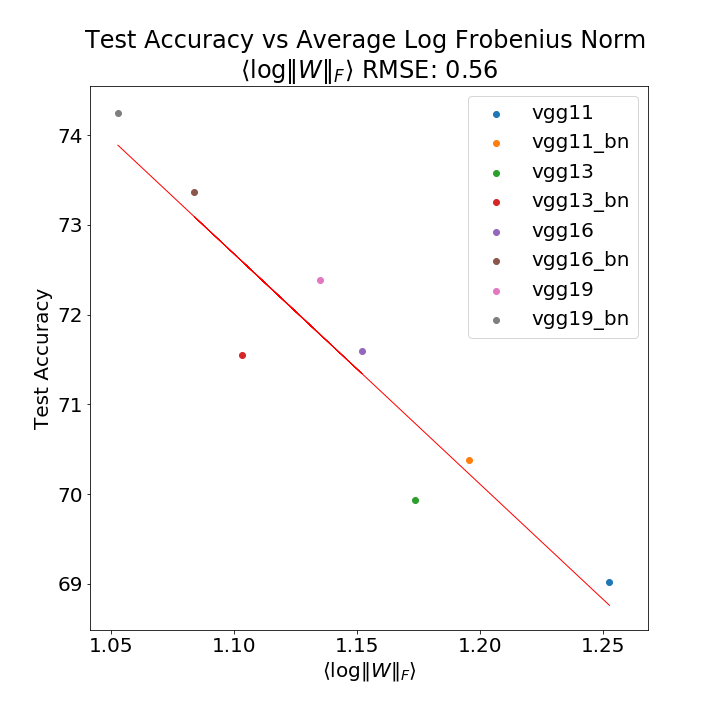
\includegraphics[width=5cm]{img/VGG_lognorm_accs.png}
        \label{fig:vgg-fnorm}
    }
    \qquad
    \subfigure[ Spectral Norm ]{
        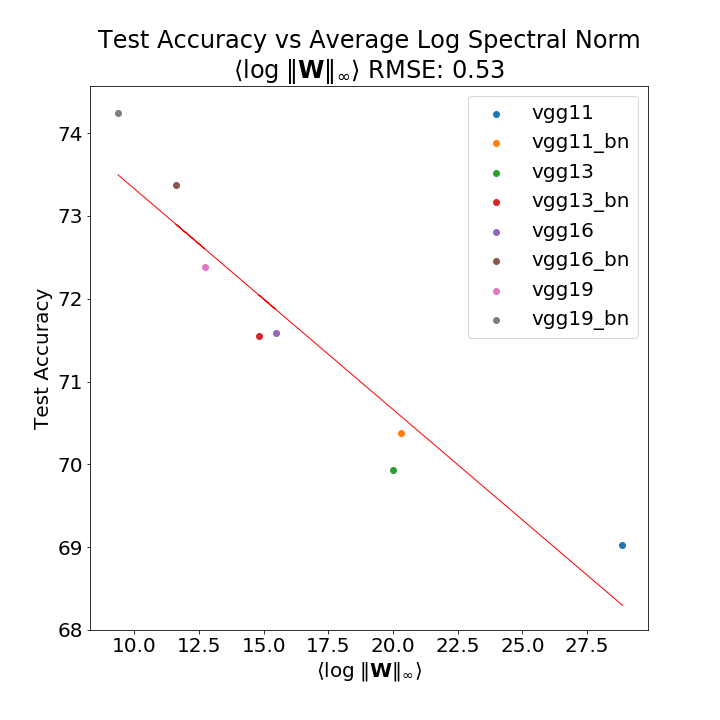
\includegraphics[width=4.9cm]{img/VGG_spectralnorm_accs.png}
        \label{fig:vgg-snorm}
    }
    \qquad
    \subfigure[ Weighted Alpha ]{
        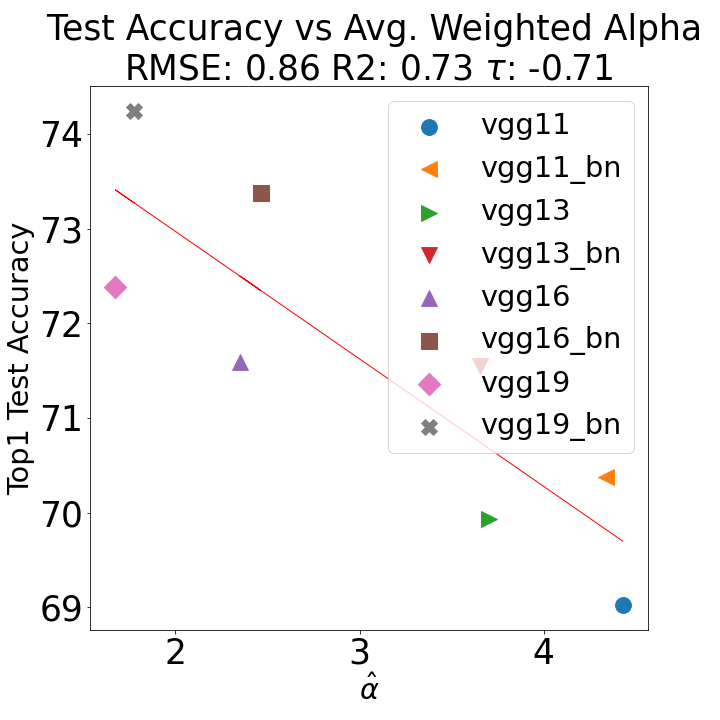
\includegraphics[width=4.9cm]{img/VGG_alpha_weighted_accs.png}
        \label{fig:vgg-walpha}
    }
    \qquad
    \subfigure[ Alpha-Norm ]{
        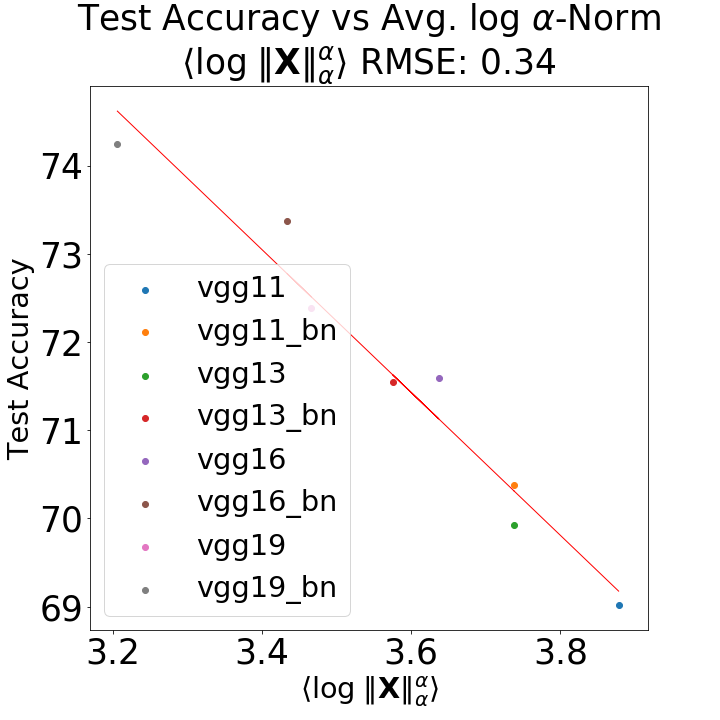
\includegraphics[width=4.9cm]{img/VGG_logpnorm_accs.png}
        \label{fig:vgg-pnorm}
    }
    \caption{Comparison of norm metrics vs reported test accuracy for pretrained VGG models, trained on ImageNet, available in pyTorch.  Plots will be updated and replace }
    

    \label{fig:vgg-metrics}
\end{figure}


Table \ref{table:cv-models} summarizes results from linear regressions, applied to the VGG, ResNet, ResNet-1K, and DenseNet series,
and reports the RMSE for all four product norm metrics.  For all series, all four metrics correlates remarkably well with
the reported Top1 test accuracies.  Moreover, the $\alpha$-Norm and/or the approximate Weighted Alpha metrics perform best.

For a more visual depiction, Figure \ref{fig:cv2-accuracy} displays the log $\alpha$-Norm metric  $\log\Vert\mathbf{W}\Vert)_{\infty}^{\infty}$ 
versus test accuracies for the ResNet, ResNet-1K, and DenseNet series. Notice that ResNet series, which has been trained on the full
ImageNet dataset, has an RMSE of $0.66$, whereas the ResNet-1K series, which has been trained on the much smaller ImageNet-1K dataset,
also correlated wells, but has a much larger RMSE of $1.9$.


\begin{figure}[t]
    \centering

    \subfigure[ ResNet ]{
        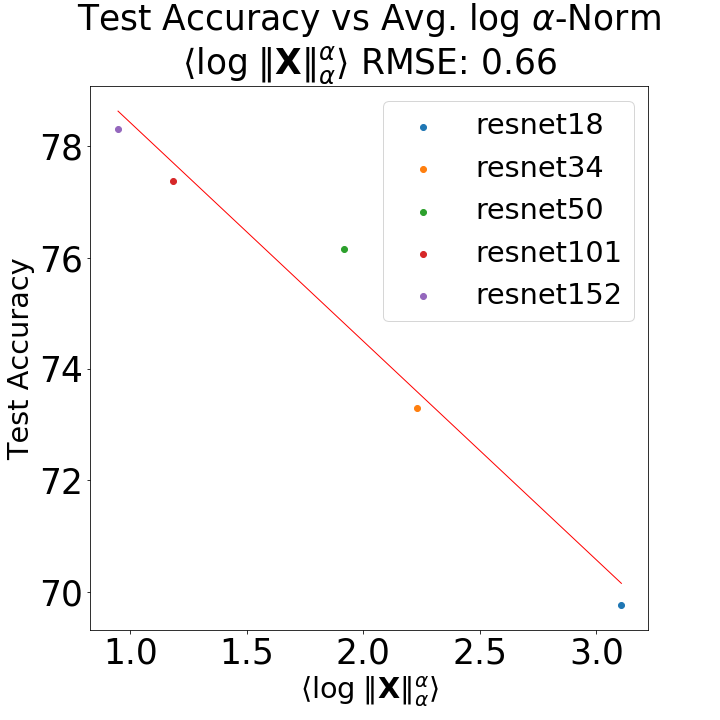
\includegraphics[width=4.2cm]{img/ResNet_logpnorm_accs.png}
        \label{fig:resnet-accuracy}
    }
    \qquad
    \subfigure[ ResNet-1K ]{
        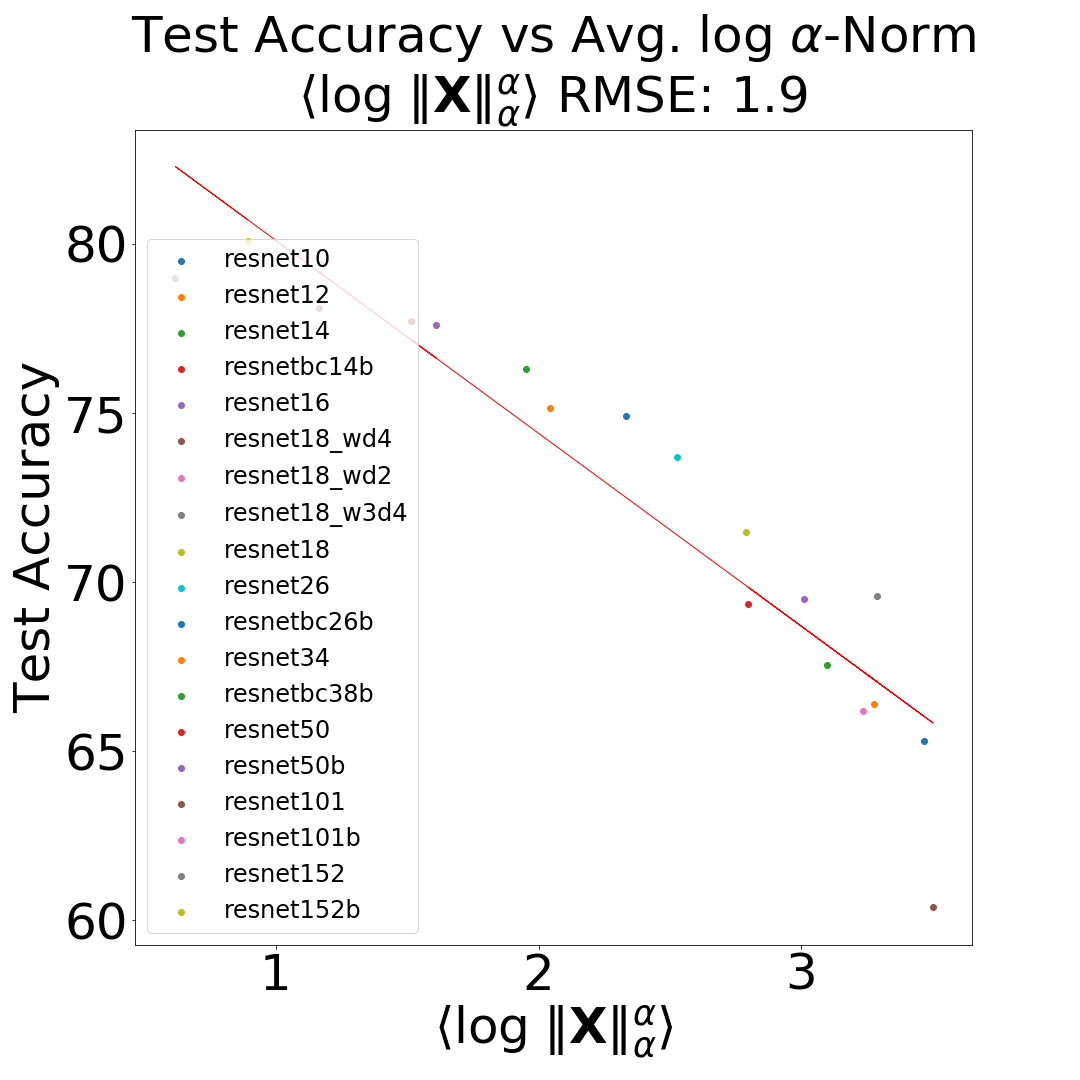
\includegraphics[width=4.5cm]{img/ResNet-1K_logpnorm_accs.png}
        \label{fig:resnet1k-accuracy}
    }
    \qquad
    \subfigure[ DenseNet ]{
        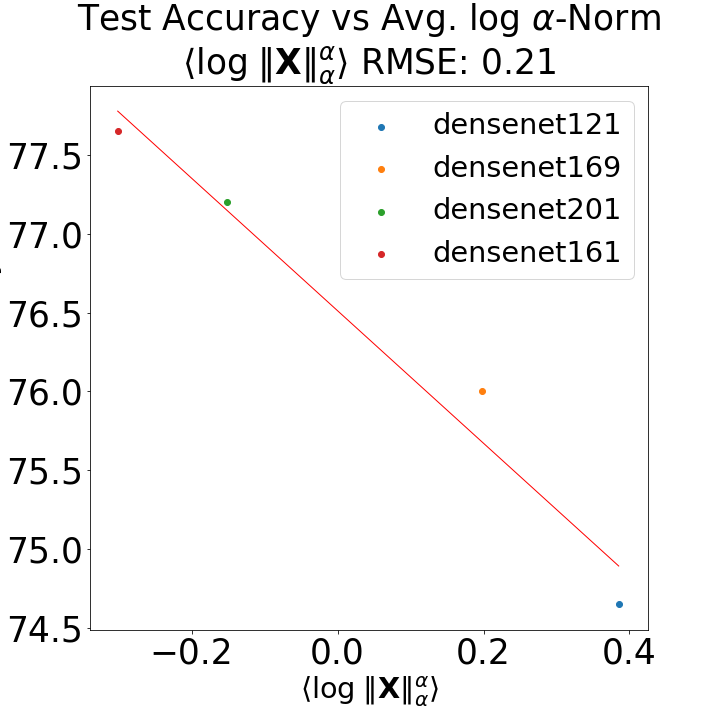
\includegraphics[width=4.4cm]{img/DenseNet_logpnorm_accs.png}
        \label{fig:densenet-accuracy}
    }
    \caption{$\alpha$-Norm vs reported Top1 Error for  ResNet, ResNet-1K, and DenseNet models}
    \label{fig:cv2-accuracy}
\end{figure}


\begin{table}[t]
\small
\begin{center}
\begin{tabular}{|p{1in}|c|c|c|c|c|}
\hline
   &    & Frobenius Norm & Spectral Norm & Weighted Alpha & Alpha-Norm \\
 Series & \#Models   & $\Vert\mathbf{W}\Vert_{F}$ & $\Vert\mathbf{W}\Vert_{\infty}$ & $\hat{\alpha}=\alpha\log\lambda_{max}$ & $\Vert\mathbf{X}\Vert^{\alpha}_{\alpha}$ \\
\hline
 VGG & 6 & 0.56 & 0.53 & 0.48 & 0.42  \\
 ResNet & 5 & 0.9 & 1.4 & 0.61 & 0.66  \\
 ResNet-1K & 19 & 2.4 & 3.6 & 1.8 & 1.9  \\
 DenseNet & 4 & 0.3 & 0.26 & 0.16 & 0.21 \\
\hline
\end{tabular}
\end{center}
\caption{RMSE for Linear Fits of Metric to Reported Top1 Test Error for all pre-trained models in the architecture series.  All models trained on ImageNet except ResNet-1K, which was trained on ImageNet-1K. }
\label{table:cv-models}
\end{table}


\paragraph{Correlation Flow in CV Models}

We can learn even more about how a pretrained model will perform by examining what we call the
\emph{Correlation Flow} down the layers.  By this, we mean the values of individual Heavy Tailed
Power Law exponent $\alpha$ for each layer weight matric $\mathbf{W}$, as a function of depth
(or layer id) in the network. (The first layer corresponds to the data, and the last layer the labels).
Figure \ref{fig:vgg-alpha-layers} plots $\alpha$ for each layer for the VGG (no batchnorm), RseNet-1K, and DenseNet models,
including the least accurate and most accurate model in each series. 

First observe that in the VGG models, $\alpha$ systematically increases as we move down the network from data to labels,
in the Conv2D layers, starting with $\alpha\le 2.0$ and reaching all the way to $\alpha\sim 5.0$.
Then, $\alpha\in[2,2.5]$ stabilizes back down to last three, large,  fully connected (FC) layers. 
In contrast, in the larger ResNet-1K (152) model, $\alpha$ remaims stable at $\alpha\sim 2.0$ all the way
until we reach the final layers.  Finally, in the DenseNet models, as in the VGG models, $\alpha$ increases
as the layer id increases, although it displays a large variance, and can range all the way to $alpha\le 8.0$.

\charles{INTERPRET}


\begin{figure}[t]
    \centering

    \subfigure[ VGG ]{
        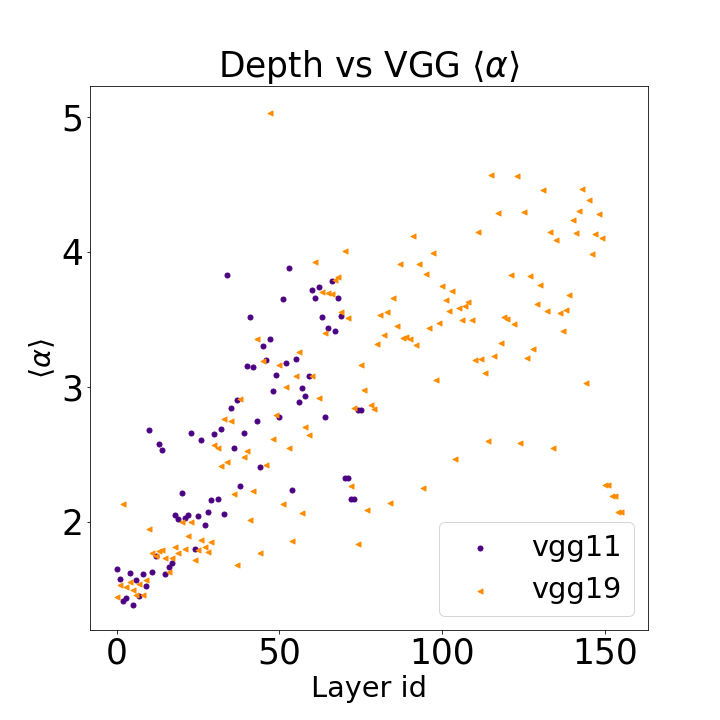
\includegraphics[width=4.5cm]{img/VGG_fnl_alpha_depth.png} 
                \label{fig:vgg-alpha-layers}
    }
    \qquad
    \subfigure[ ResNet-1K ]{
        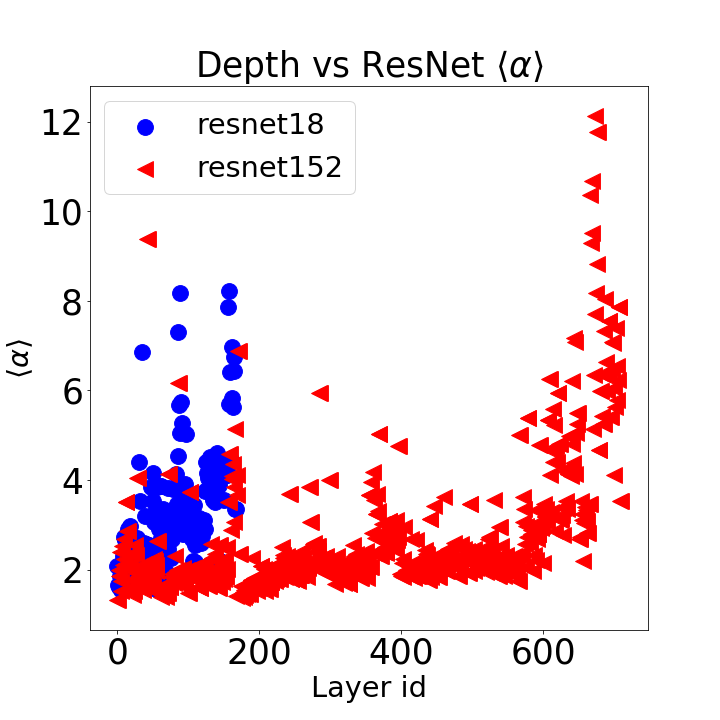
\includegraphics[width=4.5cm]{img/ResNet_fnl_alpha_depth.png} 
        \label{fig:resnet-alpha-layer}
    }
    \qquad
    \subfigure[ DenseNet ]{
        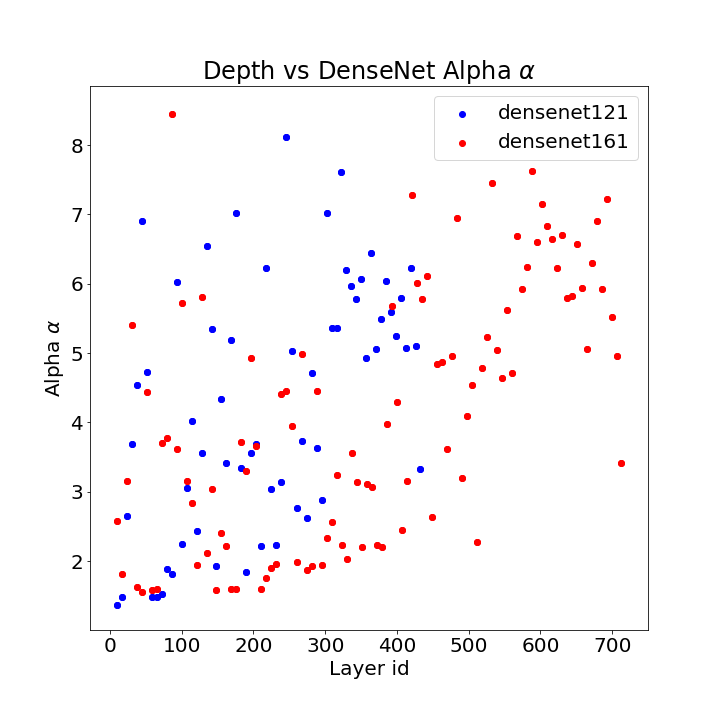
\includegraphics[width=4.5cm]{img/DenseNet_fnl_alpha_depth.png} 
        \label{fig:densenet-alpha-layer}
    }
    \caption{Correlation Flow: Heavy Tailed Power Law exponent $\alpha$ vs layer for VGG, ResNet-1K, and DenseNet models.}
    \label{fig:vgg-alpha-layers}
\end{figure}


